\begin{anexosenv}

\partanexos

\chapter{Processo de Engenharia de Requisitos}
\label{annex:processo}

\begin{figure}[!h]
        \centering
        \includegraphics[keepaspectratio=true,scale=0.24]{figuras/processo.eps}
        \caption{Processo de Engenharia de Requisitos}
\end{figure}


\chapter{Roteiro para Entrevista}
\label{annex:roteiro}

Este roteiro foi baseado no modelo disponibilizado por Fernando Firpo, disponível \href{http://analiserequisitos.blogspot.com.br/2011/07/processos-de-obtencao-de-requisitos.html}{neste link}.

\section{Parte 1 – Estabelecendo o perfil do cliente/usuário}
Previamente poderão ser pesquisadas informações como nome do entrevistado, cargo, nome da organização, ramo de atividade, entre outras informações relevantes.

\begin{itemize}
  \item Quais são as suas responsabilidades?
  \item Quais são os produtos do seu trabalho?
  \item Para que/quem (com que finalidade) você gera esses produtos?
  \item Como é medido o seu sucesso?
  \item Quais são os problemas que interferem para o sucesso de seu trabalho?
  \item Existe algo que facilita ou dificulta o seu trabalho?
\end{itemize}

\section{Parte 2 - Avaliando o Problema}
\begin{itemize}
  \item Para quais problemas faltam boas soluções?
  \item Quais são? (Continar perguntando, “Mais algum?”).
  \item Para cada problema, pergunte:
    \begin{itemize}
      \item Porque esse problema existe?
      \item Como resolvê-lo?
      \item Como você poderia resolvê-lo?
    \end{itemize}
\end{itemize}

\section{Parte 3 - Entendendo o Ambiente do Usuário}
\begin{itemize}
  \item Quem são os usuários? Os usuários são experientes nesse tipo de aplicação?
  \item Quais plataformas atualmente são usadas?
  \item Quais são os planos para a futura plataforma?
  \item Outras aplicações usadas são relevantes para essa aplicação? Se sim, fale um pouco sobre elas.
  \item Quais são as suas expectativas para a usabilidade do produto?
  \item Quais são as suas expectativas para o tempo de treinamento?
\end{itemize}

\section{Parte 4 - Recapturando para Entender}
\begin{itemize}
  \item (Listar os problemas que o cliente descreveu com suas próprias palavras).
  \item Eles representam adequadamente os problemas que você está tendo com a solução existente?
  \item Quais outros problemas, caso exista, você está enfrentando?
\end{itemize}

\section{Parte 5 - Suposições do Analista sobre o Problema do Cliente}
Validar ou invalidar suposições.

\begin{itemize}
  \item Liste quaisquer necessidades ou problemas adicionais que você acha que está preocupando o cliente ou o usuário.
    \begin{itemize}
      \item "Parece que vocês têm uma dificuldade em tal ponto…"
      \item "Será que seu problema não é tal coisa?"
    \end{itemize}

  \item Esse é um problema real?
    \begin{itemize}
      \item Quais são as razões deste problema?
      \item Como você gostaria de resolvê-lo?
      \item Qual é o peso da solução desse problema, comparado aos outros que você mencionou?
    \end{itemize}
\end{itemize}

\section{Parte 6 - Avaliando sua Solução (se aplicável)}
Resumir as principais capacidades da solução que você propôs.

\begin{itemize}
  \item O que aconteceria se você conseguisse:
    \begin{itemize}
      \item "O que aconteceria se aplicássemos essa solução?"
      \item "Como isso melhoraria o desempenho da empresa?"
    \end{itemize}
  \item "Como você classificaria cada uma dessas capacidades, por ordem de sua importância?"
\end{itemize}


\section{Parte 7 - Avaliando a Oportunidade}
\begin{itemize}
  \item Quem na sua organização precisa dessa aplicação?
  \item Quantos usuários desse tipo usariam a aplicação?
  \item O que você considera que seja uma solução bem sucedida?
\end{itemize}

\section{Parte 8 - Avaliando Necessidades de Segurança}
\begin{itemize}
  \item Quais são suas expectativas sobre a segurança?
\end{itemize}

\section{Parte 9 - Outros Requisitos}
\begin{itemize}
  \item Existe alguma necessidade legal, burocrática, ambiental, etc que deva ser atendido?
  \item Você acha que existem outros requisitos que devemos conhecer?
\end{itemize}

\section{Parte 10 - Fechamento}
\begin{itemize}
  \item Existe alguma outra questão que eu deveria ter feito?
  \item Você acredita que haja outra pessoa importante a ser entrevistada?
  \item Se depois, eu tiver alguma dúvida, posso ligar para você? Enviar e-mail? Você concorda em participar de uma revisão de requisitos?
\end{itemize}

\chapter{Roadmap Completo}
\label{annex:roadmap}

Segue-se o roadmap completo do projeto especificado. Ressalta-se que as linhas vermelhas verticais delimitam
a duração de cada PI.

\begin{figure}[!h]
        \centering
        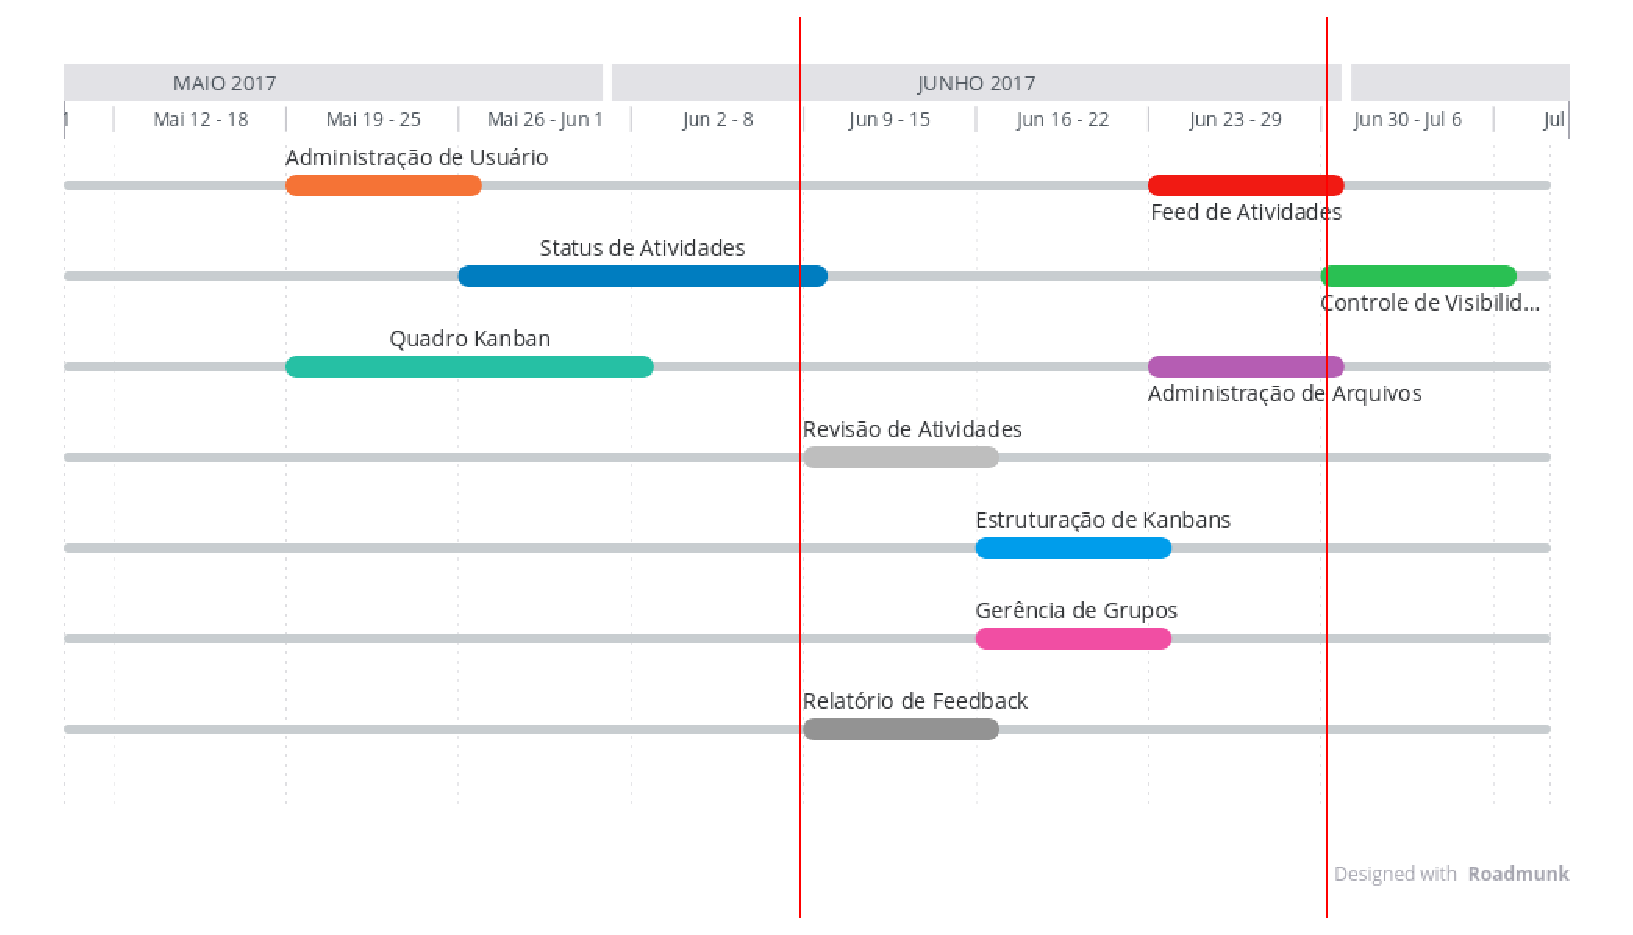
\includegraphics[keepaspectratio=true,scale=0.6]{figuras/roadmap.eps}
        \caption{Roadmap Completo}
\end{figure}


\end{anexosenv}
